\documentclass[a4paper]{article}
\usepackage{graphicx}
\usepackage{kotex}
\usepackage{verbatim}
\usepackage{mathtools}
\usepackage[a4paper, margin=1in]{geometry}


\title{AI Homework No. 4 submission}
\author{KimJaeHwan}
\date{\today}

\begin{document}

\maketitle

\section*{Problem 1e: Clustering 2D points [2 points]}
You have now completed all parts needed to run main(). Now, let’s verify your implementation by running the algorithm on 2D points. At the bottom of kmeans.py, there are codes for loading the 2D data points and the initial centroids we provided in from .csv files, and calling the main function. Run the program by typing:

\begin{verbatim}
    python kmeans.py
\end{verbatim}

\noindent
in ther terminal window. If you are successful, you should see:

\begin{verbatim}
    K-means converged after 7 steps.
\end{verbatim}

\noindent
as the output of the program. In addition, there should be 7 plots generated, in the \texttt{results/2D} folder. \textbf{Attach the 7 plot images to \texttt{submission\_studentid.pdf}}

\begin{figure}[h!]
    \centering
    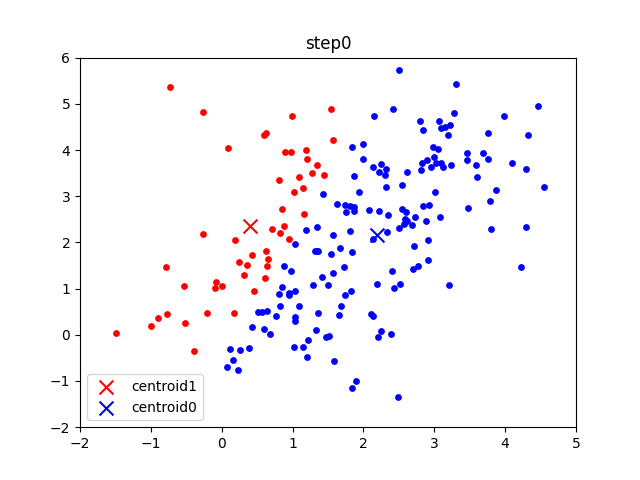
\includegraphics[width=0.327\textwidth]{../ai_assn4_prog/results/2D/step0.png}
    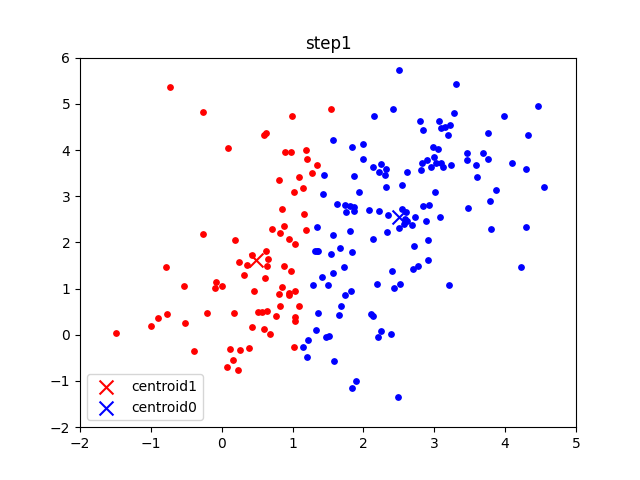
\includegraphics[width=0.327\textwidth]{../ai_assn4_prog/results/2D/step1.png}
    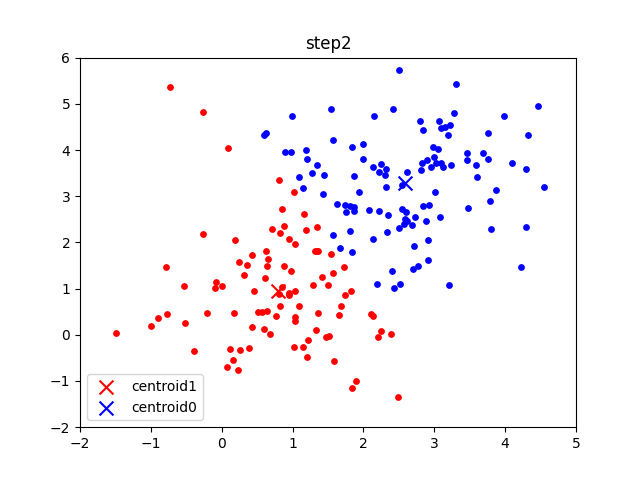
\includegraphics[width=0.327\textwidth]{../ai_assn4_prog/results/2D/step2.png}
    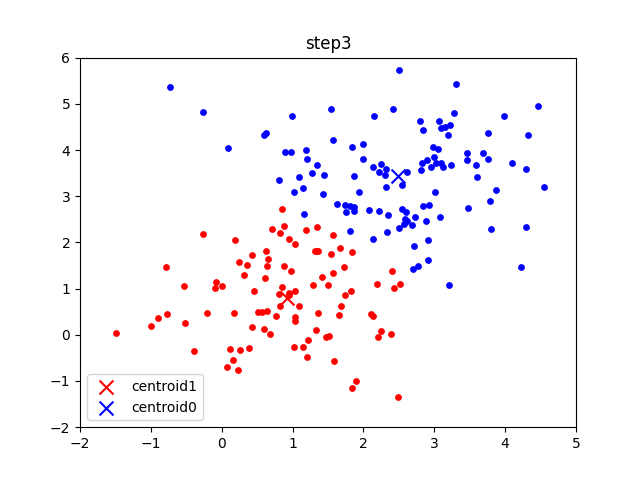
\includegraphics[width=0.327\textwidth]{../ai_assn4_prog/results/2D/step3.png}
    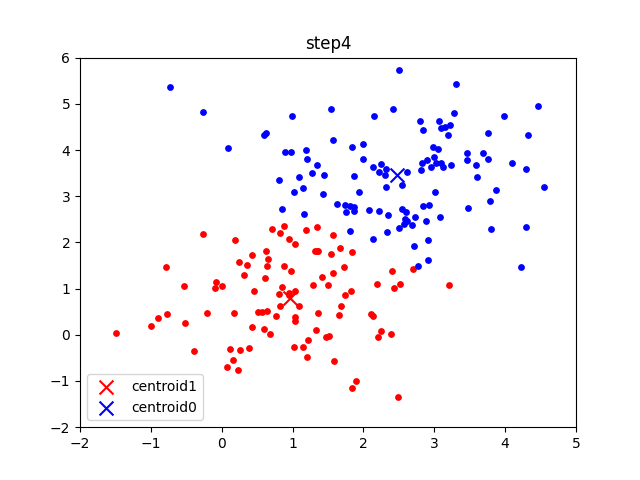
\includegraphics[width=0.327\textwidth]{../ai_assn4_prog/results/2D/step4.png}
    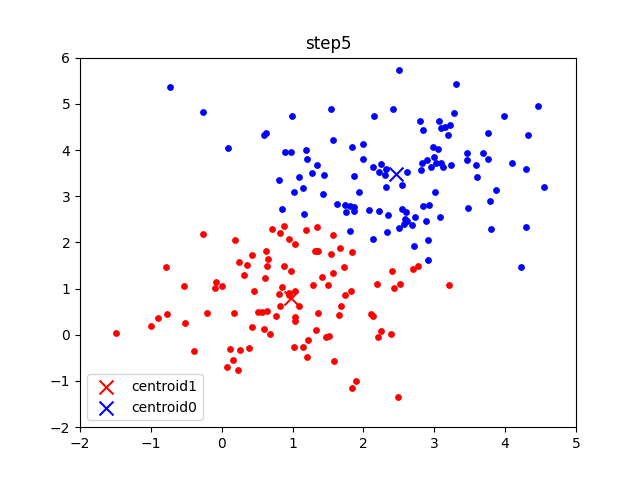
\includegraphics[width=0.327\textwidth]{../ai_assn4_prog/results/2D/step5.png}
    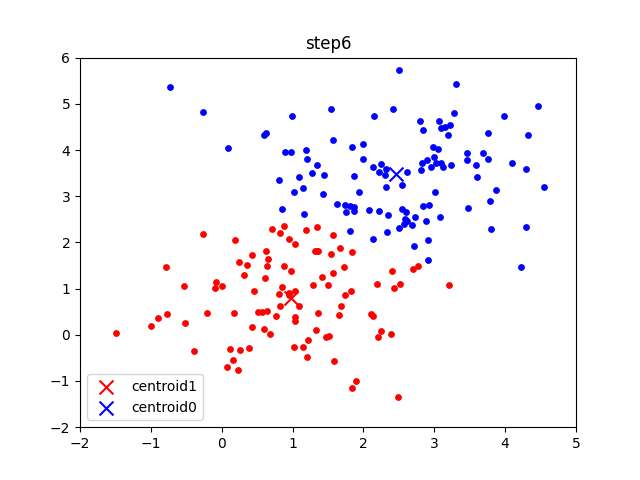
\includegraphics[width=0.327\textwidth]{../ai_assn4_prog/results/2D/step6.png}
    
\includegraphics[width=0.327\textwidth]{../white.png}
    
\includegraphics[width=0.327\textwidth]{../white.png}
    \caption{Result plots of K-mean algorithm}
    \label{fig:result}
\end{figure}

\section*{Problem 1f: Trying the Algorithm on MNIST [2 points]}
... Description of MNIST is omitted. Note \texttt{ai\_assn4.pdf} for more details

\medskip
\noindent
Why the centroid of each cluster looks like an actual digit? This question will be ungraded. But if you do not write any answers, you will get 0 points. We want you to at least think about what happened to the centroids. \textbf{Write your answers in} \texttt{submission\_studentid.pdf}.

\subsection*{Answer}

흰색인 값들의 (x, y) 좌표의 평균을 찾는 것이 아니라, 각 픽셀의 값들의 평균을 찾는 것이기 때문이다. 즉, 센트로이드 이미지의 각 픽셀은 클러스터에 포함된 이미지들의 각 픽셀의 평균값을 가지므로, 데이터포인터에서 흰색의 빈도가 높은 픽셀은 센트로이드 이미지에서도 흰색의 빈도가 높게 나타나게 된다. 따라서, 센트로이드가 실제 이미지와 유사한 형태를 띄게 된다.

\section*{Problem 2d: Clustering 2D points [2 points]}
... Description of soft K-means is omitted. Note \texttt{ai\_assn4.pdf} for more details

\medskip \noindent
Let’s compare the newly generated plots with the plots generated in Problem 1e. \textbf{Also, attach the new 7 plots to} \texttt{submission\_studentid.pdf}.

\medskip \noindent
As you may have already noticed, the hyper-parameter $\beta$ is used when calculating responsibility. Change the value of $\beta$ to 50 in main() function of \texttt{soft\_kmeans.py} file. What changes have been made to the plots? Think about how $\beta$ affects soft K-means clustering and
\textbf{write your answer with a} \texttt{step6} \textbf{plot when setting $\beta$ to 50} in \texttt{submission\_studentid.pdf}

\subsection*{Answer}

일반 k-means clustering과 다르게, soft k-means clustering에서는 $\beta$의 값에 따라서 각 클러스터의 책임도가 결정된다. $\beta$의 값을 가정하고 식을 분석해본다면, 

\begin{itemize}
    \item $\beta = 0$인 경우: 
    
    responsibility of $x_i$ to cluster $k$, 
    $$r_{ki} = \frac {\textnormal{exp}(-\beta dist_{ki})}{\sum_{l \in K} \textnormal{exp}(-\beta dist_{li})} = \frac {\textnormal{exp}(0)}{\sum_{j=1}^{K} \textnormal{exp}(0)} = \frac {1}{K}$$

    $$centroid_k = \frac{\sum_{i\in N} r_{ki}x_i}{\sum_{i \in N} r_{ki}} = \frac{\sum_{i\in N} \frac {1}{K}x_i}{\sum_{i \in N} \frac {1}{K}} = \frac{\sum_{i\in N} x_i}{N}$$

    즉, 모든 데이터 포인트가 동등하게 기여하므로, 모든 센트로이드가 데이터 포인터들의 평균 한 점으로 수렴하게 된다.

    \item $\beta \to \infty$인 경우:
    
    극한을 취하게 되면, 
    $$\textnormal{exp}(-\beta dist_{ki}) \to \begin{cases}
        1 & \textnormal{if $k$ is the nearest centroid to $i$} \\
        0 & \textnormal{otherwise}
    \end{cases}$$

    $$r_{ki} = \begin{cases}
        1 & \textnormal{if $k$ is the nearest centroid to $i$} \\
        0 & \textnormal{otherwise}
    \end{cases}$$

    로 수렴한다. 따라서, 각 데이터 포인트는 가장 가까운 센트로이드에만 책임도를 부여하게 되고, 이는 일반적인 k-means clustering과 같아진다.

\end{itemize}

\noindent
따라서, $\beta$는 가까운 데이터 포인터에 영향을 많이 받는지에 대한 가중치를 조절하는 하이퍼파라미터이다. 아래 이미지를 보면, $\beta$가 3인 경우에 비해서 $\beta$가 50인 경우 클러스터로부터 비교적 먼 경계에 위치한 데이터 포인트 또한 책임도를 부여받아 색이 진하게 나타나는 것을 확인할 수 있다.

\bigskip
\noindent
Note. The plots are attached in the next page.

\pagebreak

\begin{figure}[h!]
    \centering
    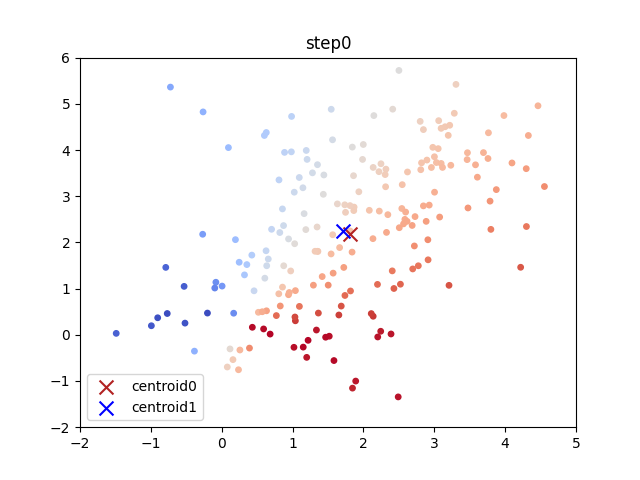
\includegraphics[width=0.327\textwidth]{../ai_assn4_prog/results/2D_soft beta=3/step0.png}
    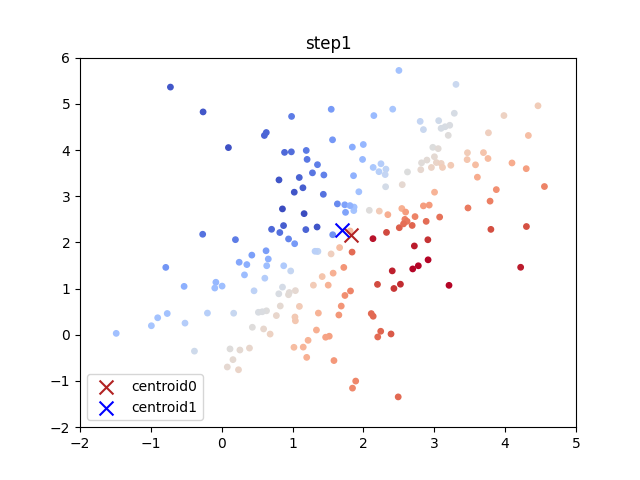
\includegraphics[width=0.327\textwidth]{../ai_assn4_prog/results/2D_soft beta=3/step1.png}
    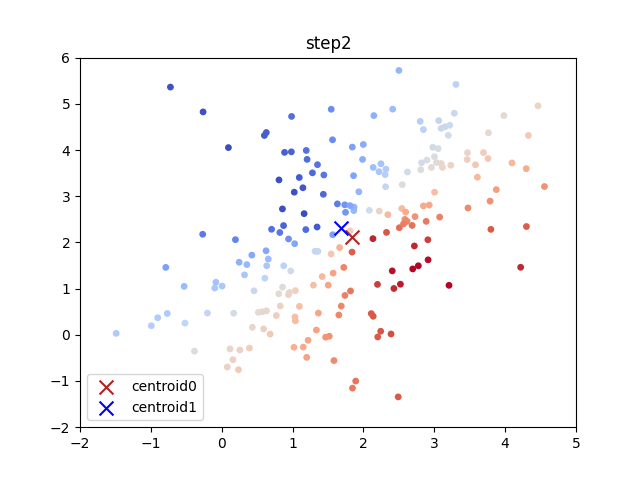
\includegraphics[width=0.327\textwidth]{../ai_assn4_prog/results/2D_soft beta=3/step2.png}
    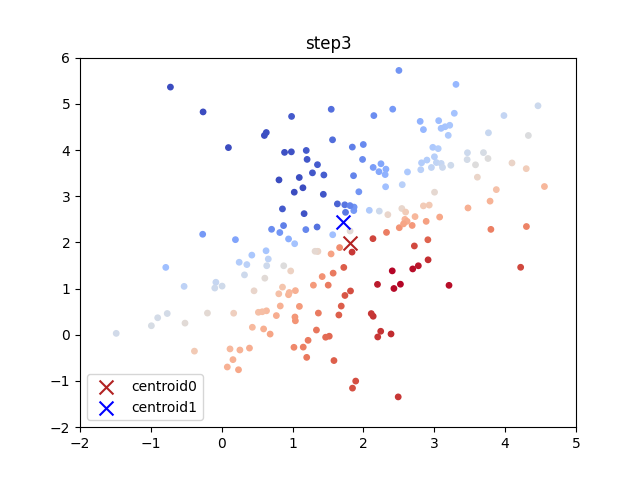
\includegraphics[width=0.327\textwidth]{../ai_assn4_prog/results/2D_soft beta=3/step3.png}
    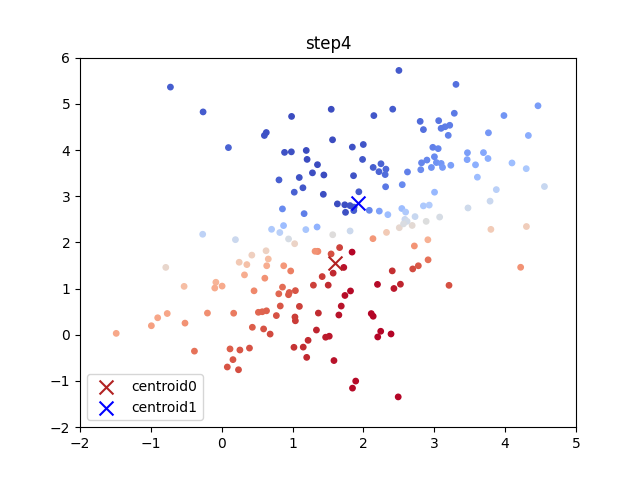
\includegraphics[width=0.327\textwidth]{../ai_assn4_prog/results/2D_soft beta=3/step4.png}
    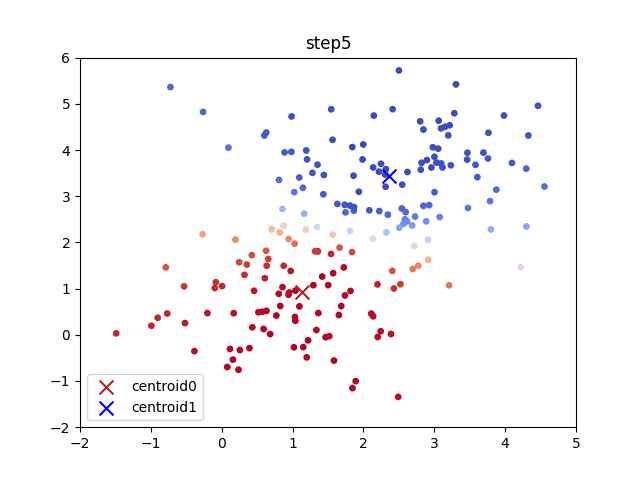
\includegraphics[width=0.327\textwidth]{../ai_assn4_prog/results/2D_soft beta=3/step5.png}
    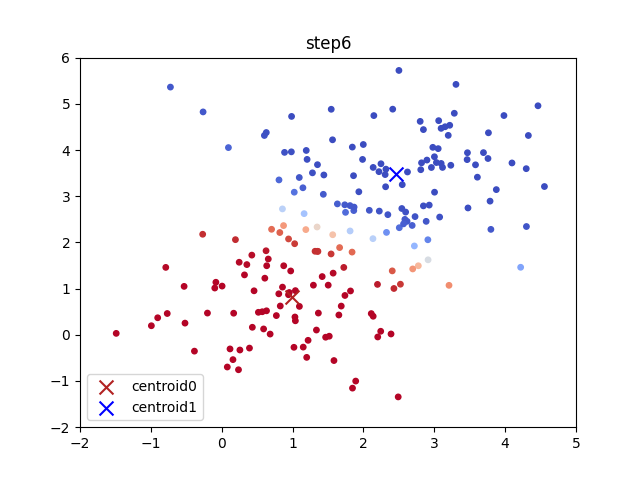
\includegraphics[width=0.327\textwidth]{../ai_assn4_prog/results/2D_soft beta=3/step6.png}
    
\includegraphics[width=0.327\textwidth]{../white.png}
    
\includegraphics[width=0.327\textwidth]{../white.png}
    \caption{Result plots of soft-K-mean algorithm}
    \label{fig:result2}
\end{figure}

\begin{figure}[h!]
    \centering
    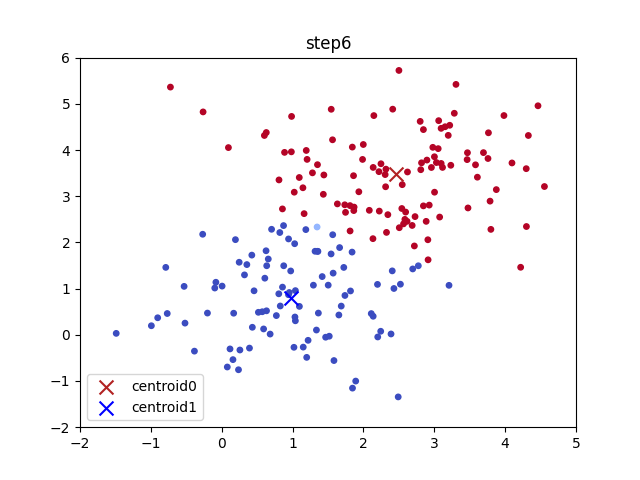
\includegraphics[width=0.8\textwidth]{../ai_assn4_prog/results/2D_soft/step6.png}
    \caption{Result plots of soft-K-mean algorithm when $\beta$ is set to 50}
    \label{fig:result3}
\end{figure}

\end{document}